\documentclass[12pt,a5]{bxjsarticle}

\usepackage{xltxtra}
\setmainfont{IPAPMincho}
\setsansfont{IPAPGothic}
\setmonofont{IPAGothic}
\XeTeXlinebreaklocale "ja"

\usepackage{hyperref}
\usepackage{listings}
\usepackage{verbatim}

\newcommand{\e}{\mathrm{e}}

\title{物理学情報処理論2 problem4}
\date{}

\begin{document}
\maketitle

$ \frac{d^2u}{d\theta^2} + u = 2 + \epsilon u^2, u(0) = 1, \frac{du}{d\theta}(0) = 0 $

\section{}
この方程式を $ \epsilon = 0, 0.001, 0.01, 0.1 $ の場合に解いたものは以下の図のようになる。
Symplectic法を用いて数値的に解いた。

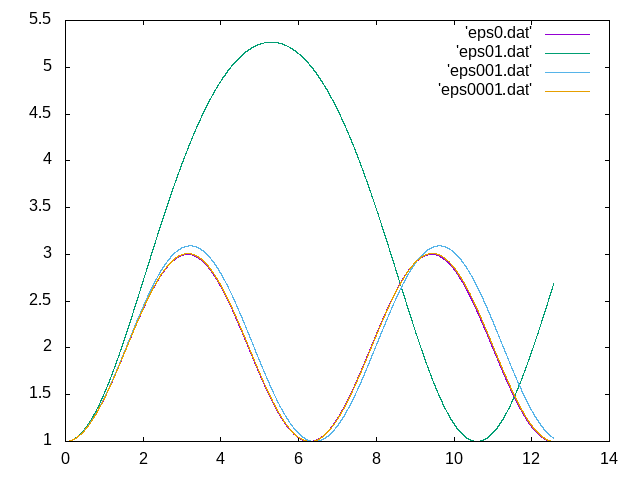
\includegraphics[width=\linewidth]{orbit.png}

\section{}
上記の解の周期$ T $について、$ T - 2\pi $を両対数グラフに描くと以下のようになる。
$\epsilon$の小さな範囲において、両対数グラフで直線上になっていることから、
これは傾きを$ \alpha $とすると$ O(\epsilon^\alpha) $のような関数となっていることがわかる。

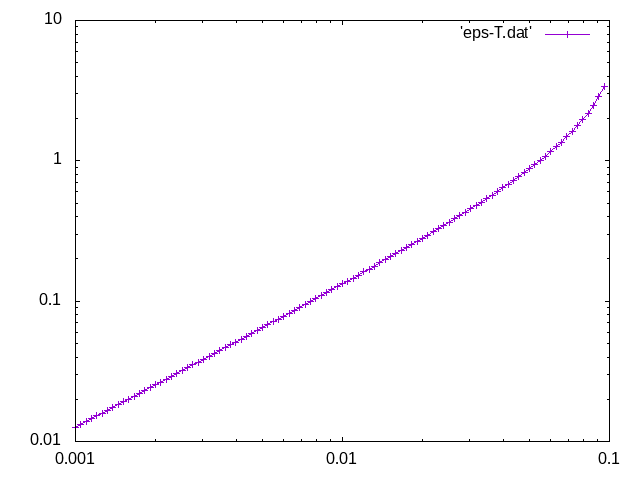
\includegraphics[width=\linewidth]{T.png}

以下のスクリプトを用いて、orbit.datから図を生成した。
\lstinputlisting[caption=plot.sh,language=bash]{plot.sh}

\end{document}
